\chapter*{About provable reproducibility}
\label{chp:0-reproducibility}

Provable reproducibility is an initiative I hereby launch, which pursues the
goal of making results found in articles, theses, and software packages easy to
reproduce and verify. No ambiguity, no data manipulation, no cherry-picked
parameters, and no hand-crafted results. Every figure, plot, table, formula, and
text in a provably reproducible project can be unequivocally traced back to where
it originated from. This goes one step further than merely uploading the
source code of a project, where a reviewer or user will have to go through the
tedious and often error-prone process of reproducing the results.\\

The proof is delivered by openly -- not locally -- recreating every aspect of a
project in an online archive. This includes, but is not limited to
\begin{itemize}
    \item downloading, importing or creating all the external dependencies which are being used (code, data, \dots);
    \item running all the computations and generating the corresponding results (plots, tables, \dots);
    \item and building the project outcome (article, report, \dots).
\end{itemize}
Such a reproduction pipeline can be implemented without too much effort by
using a CI/CD framework available in most contemporary software development
and version control services, such as GitHub and GitLab.

\vfill
\begin{center}
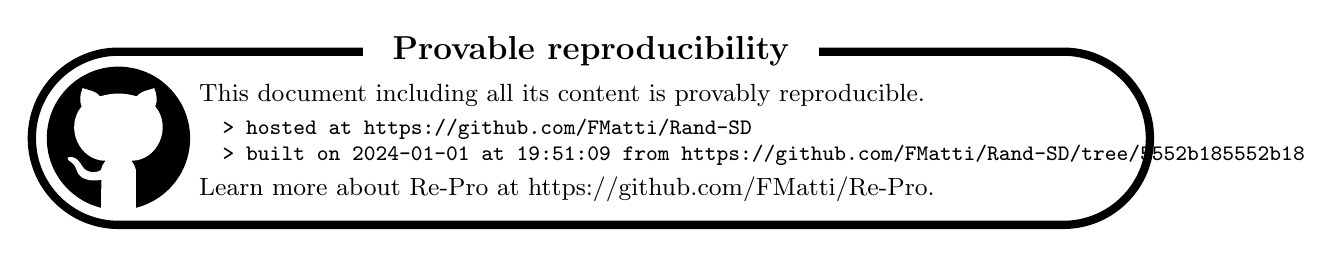
\begin{tikzpicture}
    \begin{scope}[scale=0.13]
        % Background
        \fill[black] (0, 0) circle (7);

        % Foundation
        %\fill[white] (-3.2, -5.3) rectangle (3.2, -4.7);

        % Logo
        \fill[white] (1.7, -7.3) -- (-1.7, -7.3) to[out=90, in=270] (-1.675, -4.05)
                                                 to[out=190, in=330] (-3.6, -3.8)
                                                 to[out=150, in=330] (-4.6, -2.35) % Tail
                                                 to[out=150, in=280] (-5.0, -1.9) % Tail
                                                 to[out=20, in=140] (-4.0, -2.1) % Tail
                                                 to[out=320, in=160] (-3.0, -3.2) % Tail
                                                 to[out=340, in=210] (-1.7, -3.1) % Tail
                                                 to[out=80, in=230] (-1.25, -2.2) % Shoulder (left)
                                                 to[out=180, in=230, looseness=1.15] (-3.6, 3.1) % Cheek (left)
                                                 to[out=110, in=250] (-3.5, 4.9) % Ear (left)
                                                 to[out=340, in=130] (-1.8, 4.1) % Ear (left)
                                                 to[out=15, in=165] (1.8, 4.1) % Top
                                                 to[out=50, in=200] (3.5, 4.9) % Ear (right)
                                                 to[out=290, in=70] (3.6, 3.1) % Ear (right)
                                                 to[out=310, in=0, looseness=1.15] (1.25, -2.2) % Cheek (right)
                                                 to[out=310, in=100] (1.7, -3.1) % Shoulder (right)
                                                 -- cycle;
    \end{scope}
    \draw[black, line width=3] (0, 1.1) to (12, 1.1) arc (90:-90:1.1) to (0, -1.1) arc (270:90:1.1);
    \fill[white] (3.1, 1.0) rectangle (8.9, 1.2);
    \node at (6, 1.1) {\bfseries \large Provable reproducibility};
    \node[anchor=west] at (0.9, 0.55) {\small This document including all its content is provably reproducible.};
    \node[anchor=west] at (1.2, 0.12) {\footnotesize \texttt{> hosted at \url{https://github.com/FMatti/Rand-SD}}};
    \node[anchor=west] at (1.2, -0.22) {\footnotesize \texttt{> built on 2024-01-01 at 19:51:09 from \href{https://github.com/FMatti/Rand-SD/tree/5552b18}{5552b18}
}};
    \node[anchor=west] at (0.9, -0.65) {\small Learn more about Re-Pro at \url{https://github.com/FMatti/Re-Pro}.};
\end{tikzpicture}
\end{center}
